% Present experiments, metrics, and results.
% Use tables (\begin{table}...\end{table}) and figures where appropriate.
% \begin{table}[h!]
%     \centering
%     \begin{tabular}{|c|c|}
%         \hline
%         Category & Score \\
%         \hline
%         Coolness & 31.1 \\
%         Cuteness & 15.2 \\
%         Toughness & 1.15 \\
%         Elasticity & 87.5 \\
%         \hline
%     \end{tabular}
%     \caption{Features of Ipsum}
%     \label{tab:placeholder}
% \end{table}
% See \cref{tab:placeholder}.

\begin{figure}
    \centering
    \includegraphics[width=\linewidth,height=.95\textheight,keepaspectratio]{figures/mn_reuse_blocked_flowchart.png}
    \caption{Tiled and Blocked Harness Flowchart}
    \label{fig:tiledandblockedharnessumldiagram}
\end{figure}


\subsection{Experimental Setup and Metrics}
% fixed machine configuration
% 1024x1024 GEMM, 32x32 tiles, fp16
% what is tiling, why do we need it
% How is job scheduling and allocation done (ScratchpadLayoutAllocator, BlockTileJob, whatever is used in both naive and tiled)
% What is held constant across experiments
% Which metrics are reported: cycles, bytes_transmitted, flops, bandwidth, queue depths, utilization
% brief note on correctness checks
\Cref{fig:tiledandblockedharnessumldiagram} shows the structure of the shared platform used by the naive and blocked harnesses. All experiments evaluate a $1024 \times 1024$ fp16 GEMM decomposed into $32 \times 32$ tiles, which yields $32$ tiles per matrix dimension, $1024$ output tiles and $32\times1024$ tile-pair GEMMs in total. However, the working set does not fit on chip: the scratchpad capacity is 2 MB, whereas the two input matrices alone occupy 4 MB at fp16 precision. Additionally, the modeled systolic-array compute kernel operates on one $32 \times 32$ tile GEMM at a time. Thus, the larger matrix must be expressed as a sequence of tile jobs with explicit staging and accumulation: it is necessary for our system to kernelize the workload to be able to process the sheer amount of data.

At the harness level, both schedules operate on explicit tile-granular jobs and explicit scratchpad staging locations while advancing the machine cycle by cycle and checking for tile completion through queue and pipeline state. The blocked reuse schedule introduced later extends this same baseline structure with a richer block-level layout policy.

The reported metrics are chosen to capture both throughput and where that throughput is lost. Total cycles and average per-output-tile latency measure end-to-end progress. \texttt{bytes\_transmitted} reports VLS-visible traffic across the scratchpad--vector-core boundary, while \texttt{bytes\_internal} reports useful internal systolic array traffic. The evaluation also reports modeled floating-point work, throughput in operations per cycle, external and internal bandwidth, MAC utilization over both valid-MAC windows and the full run, and time-averaged and peak queue occupancies along the critical paths. Correctness is checked against a reference fp16 accumulation, with maximum and mean absolute error reported for the full output matrix.

\begin{figure}
    \centering
    \includegraphics[width=\linewidth,height=.95\textheight,keepaspectratio]{figures/gemm2a.png}
    \caption{Kenelization a GEMM with Tiling \cite{cnugterenOpenCLMatrixmultiplication}}
    \label{fig:tilegemm}
\end{figure}

\subsection{Naive 1024x1024 Tiled GEMM Baseline}
% workload and scheduling policy in test_scratchpad_vector_core_sysarr_tpu_tiled_1024.py
% row-major output-tile schedule
% double-buffered tk prefetch
% one tk job computes at a time
% vector-core accumulation path
% headline baseline numbers
The naive baseline follows a strictly tiled schedule on the output coordinates $(t_i, t_j)$. One output tile $C[t_i, t_j]$ is completed in full before the harness advances to the next tile. Within each output tile, the reduction dimension $t_k$ runs from $0$ to $31$ and is staged through two prefetch slots for double buffering. When a slot becomes free, the next available $t_k$ job is launched into it, but only one GEMM tile is allowed to occupy the compute path at a time. The two slots therefore overlap preload with compute, but they do not allow concurrent systolic-array execution.

A partial output row returned through the GSAU triggers a scratchpad load of the current accumulator row, an element-wise add in the \texttt{VectorDatapath}, and a store of the updated row back to the scratchpad accumulator tile. After all $32$ $t_k$ contributions have been folded into that accumulator tile, the finished output tile is drained to DRAM. Therefore, the baseline exposes the forward feed into the systolic array: load, response, accumulation, and store traffic required to turn partial rows into a final output tile.

\begin{table}[ht]
\centering
\caption{Headline metrics for the naive tiled $1024 \times 1024$ GEMM baseline.}
\label{tab:naive-baseline}
\begin{tabular}{ll}
\toprule
\textbf{Metric} & \textbf{Value} \\
\midrule
Total simulation cycles & 22M \\
Avg.\ cycles per output tile & 22{,}390.4 \\
Avg.\ tile-GEMM cycles & 406.03 \\
Avg.\ SDMA load cycles & 945.56 \\
Avg.\ systolic-array compute cycles & 76.0 \\
Avg.\ valid-MAC cycles & 71.0 \\
Modeled floating-point ops & 10{,}332M \\
Throughput (FLOP/cycle) & 450.64 \\
VLS-visible bytes transmitted & 268M \\
Useful system-internal bytes & 4{,}077M \\
External bandwidth (avg.) & 11.71 B/cycle \\
External bandwidth (active) & 64.50 B/cycle \\
MAC utilization (full run) & 4.57\% \\
MAC utilization (valid-MAC window) & 45.07\% \\
Max absolute error & 0.0 \\
\bottomrule
\end{tabular}
\end{table}

Errors, saturation, and overflow remain zero. The baseline is therefore correct and locally compute-dense, but not end-to-end efficient.

\subsection{Baseline Bottleneck Analysis}
% explain why the naive schedule is slow
% preload-limited behavior
% compute gaps between tk jobs
% accumulator traffic overhead
% queue-depth evidence
% systolic-array utilization evidence
% use gantt/cycle breakdown here

The baseline is limited by preload pacing: one output tile costs about $22{,}390$ cycles, whereas the $32$ measured tile-GEMM windows contribute only about $12{,}993$ cycles of direct compute. For the first output tile, $t_k^0$ and $t_k^1$ launch at cycle $0$, but computation does not begin until cycle $969$ when the first preload becomes ready. After that warmup, the machine repeatedly alternates between a short compute window and a much longer slot-refill interval.

The reused slot for $t_k^2$ is relaunched at cycle $1375$ but does not become preload ready until cycle $2331$, so the refill takes $956$ cycles while the tile of the opposite slot GEMM occupies the compute path for only about $406$ cycles, showing that the schedule is imbalanced. Double buffering still overlaps part of the Scratchpad Direct Memory Access (SDMA) load with compute, but it cannot hide a refill interval that is more than twice as long as the compute window. The result, visible in \cref{fig:naive-gantt}, is a system that computes densely in bursts and then waits for the next tile.

At the VLS-visible boundary, activation and weight fetches contribute 134M bytes in total, and the remaining 134M of the measured 268M transmitted bytes comes from accumulator-row movement alone. Queue data supports the same story: scheduler packet occupancy stays negligible, while the GSAU read queue and VLSU destination FIFO show more persistent pressure deeper in the return and load paths. This is why the baseline reaches 45.07\% utilization over valid-MAC windows but only 4.57\% over the full run. The system is therefore limited by staged data movement and accumulation support.

\begin{figure}
    \centering
    \includegraphics[width=\linewidth,height=.95\textheight,keepaspectratio]{figures/kernel_gantt_ti00_tj00.png}
    \caption{Tagged microkernel Gantt for the first output tile. Long SDMA preload spans dominate the shorter compute windows and create repeated bubbles.}
    \label{fig:naive-gantt}
\end{figure}

\subsection{Blocked M/N Reuse Scheduling}
% scheduling idea in test_scratchpad_vector_core_sysarr_tpu_tiled_1024_blocked_mn.py
% define weight_reuse_m and activation_reuse_n as block dimensions over output tiles
% explain block-level weight-stationary execution and what remains the same vs the naive baseline
% use the blocked-harness schedule/presentation figures to show one block and one reuse pass
% end by stating the expected effect: less reload traffic per output tile and better overlap, not a new machine model

The blocked schedule changes the harness policy. In a fixed reduction tile $t_k$, the harness groups work in reuse blocks that preload a small set of weight tiles and a larger set of activation tiles into staging buffers supported by the scratchpad. It then executes a weight-stationary loop: one resident weight tile is loaded into the systolic array path, the queued activation tiles are streamed through it back-to-back, the resulting partial sums are folded into the accumulator tile through the same return path used by the naive baseline, and only then does the harness advance to the next resident weight tile. For each $(t_i\_\text{block}, t_j\_\text{block}, t_k)$ block, it preloads $N$ activation tiles and $M$ weight tiles, loads one resident weight tile into the systolic array, and streams the activation tiles before flushing and repeating.

For the measured blocked run used throughout this section, the policy is $m2\_n32$: each reuse block holds $2$ resident weight tiles and streams $32$ activation tiles. The schedule log reflects that structure. The blocks start at $(t_i^0, t_j^0)$, complete, then advance by two columns of the output-tile before repeating; after 64 such column blocks, the harness advances by 32 output-tile rows. The blocked schedule therefore covers a fixed-$t_k$ output region in coarse blocks rather than completely finishing one output tile before moving on. The performance change therefore comes from a different staging policy and reuse pattern.

\subsection{Analytical Reuse Intuition}
% use the smart_tile_scheduling notebook only for intuition, not for final measured claims
% show how larger M/N reuse moves the schedule from refill-dominated to more compute-dense execution
% use the notebook timelines/utilization surfaces to explain why reuse helps under finite bandwidth
% call out the notebook simplifications explicitly before transitioning back to measured simulator data

\Cref{fig:mn-util-surface} presents the simplified notebook model's predicted MAC utilization as a function of weight reuse $M$ and activation reuse $N$ at a fixed external bandwidth of 32 bytes per cycle. The surface is useful for intuition, but it should be read qualitatively rather than as an end-to-end performance bound: it omits scratchpad bank contention, round-trip psum reload/store traffic, and queue-induced backpressure. Under that simplified load/compute/drain view, reuse helps because one operand fill can cover a longer burst of back-to-back tile GEMMs before the next refill.

However, doubling reuse depth does not imply near-saturation. A burst that performs only two tile-GEMMs still pays both a fill and a drain phase, so its MAC utilization remains bounded near one half rather than jumping to the mid-90\% range. Larger reuse depths continue to extend the compute burst, but the gains taper gradually and approach saturation only asymptotically. The analytical surface is therefore best interpreted as showing the direction of improvement with more reuse, not as proving that moderate reuse factors eliminate the memory-side overheads of the real machine.

The main value of the analytical surface is directional. Increasing activation-side reuse $N$ lowers the frequency of weight reloads, while increasing weight-side reuse $M$ widens the set of resident weights that can be paired without an intervening refill. Both effects reduce refill-dominated gaps and create a deeper pool of ready work behind each scratchpad resident tile. In this bandwidth-limited regime, the notebook suggests that activation-side reuse moves the surface more strongly, but the measured simulator data remains the authoritative source for absolute MAC-utilization values because the notebook does not model the accumulator path or other machine-level service stalls.

\begin{figure}
    \centering
    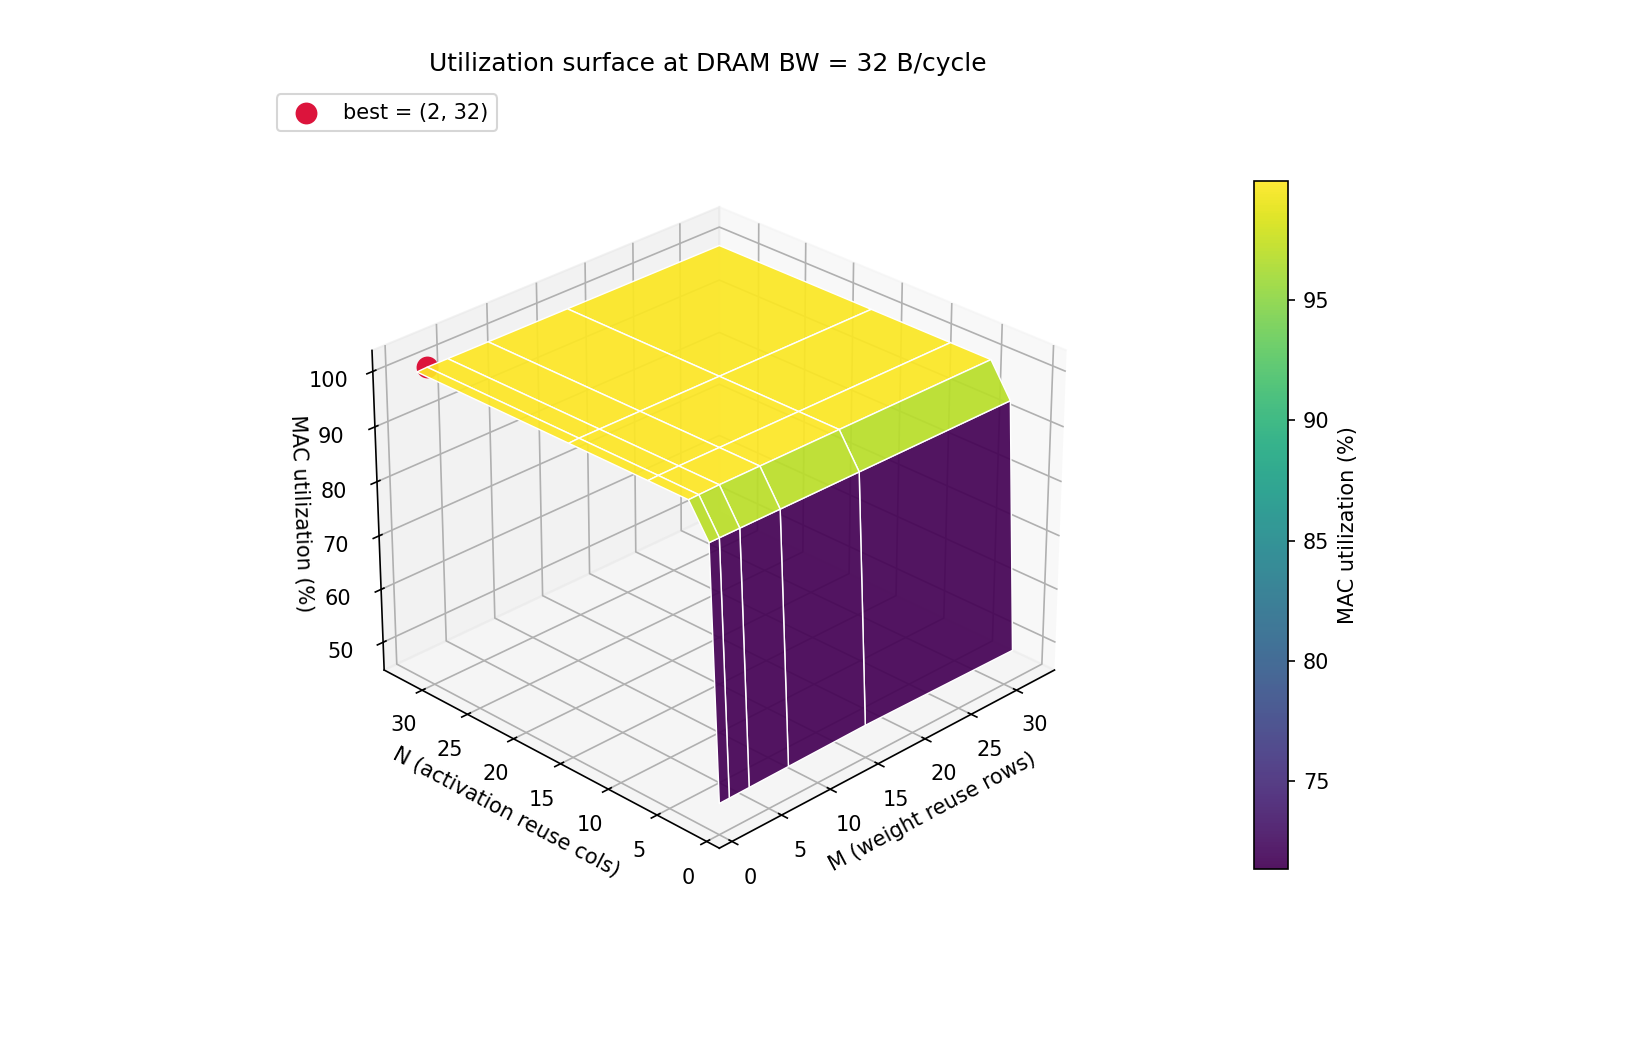
\includegraphics[width=\linewidth,height=.95\textheight,keepaspectratio]{figures/mn_utilization_surface_bw32.png}
    \caption{Derived MAC-utilization surface for the simplified notebook model at $32$ B/cycle DRAM bandwidth. It should be read as a qualitative reuse trend rather than an end-to-end utilization prediction.}
    \label{fig:mn-util-surface}
\end{figure}

\subsection{Measured Reuse-Policy Comparison}
% compare Naive, m2_n4, m2_n8, m4_n4, and m4_n8 using the measured blocked_mn_reuse_1024 results
% focus on cycles, bytes_transmitted, throughput, arithmetic intensity, and active/full-run utilization
% identify which policies reduce external traffic the most and which deliver the best end-to-end speedup
% this is the main measured comparison table/plot subsection

For cross-policy comparison, throughput is reported algorithmically as fixed GEMM FLOPs divided by total cycles. Unlike microarchitectural floating-point counts, which vary with how much accumulator traffic and other internal work each schedule generates, this measure stays invariant across schedules and therefore supports a cleaner end-to-end comparison. \Cref{tab:reuse-policy-comparison} shows that every blocked policy improves on the naive baseline in cycles, external traffic, and utilization.

\begin{table}[ht]
\centering
\small
\caption{Measured policy comparison. The naive row uses the tiled baseline from this evaluation; the $m8\_n32$ point uses the measured queue-size-4 run from the scratchpad-frontend queue sweep.}
\label{tab:reuse-policy-comparison}
\resizebox{\columnwidth}{!}{
\begin{tabular}{lrrrrrr}
\toprule
Policy & Cycles & Bytes & Algo tput & Ext. AI & Full util. & Active util. \\
 & (M) & (M) & (FLOP/cycle) & (FLOP/B) & (\%) & (\%) \\
\midrule
Naive & 22.93 & 268 & 93.66 & 8.00 & 4.57 & 45.07 \\
$m2\_n4$ & 15.36 & 218 & 139.78 & 9.85 & 6.83 & 78.05 \\
$m2\_n8$ & 12.95 & 210 & 165.86 & 10.24 & 8.10 & 87.67 \\
$m4\_n4$ & 13.25 & 218 & 162.07 & 9.85 & 7.91 & 78.05 \\
$m4\_n8$ & 11.97 & 210 & 179.38 & 10.24 & 8.76 & 87.67 \\
$m2\_n32$ & 12.67 & 203 & 169.51 & 10.56 & 8.28 & 96.60 \\
$m8\_n32$ & 11.22 & 203 & 191.44 & 10.56 & 9.35 & 96.60 \\
\bottomrule
\end{tabular}
}
\end{table}

Increasing activation reuse from $n=4$ to $n=8$ reduces VLS-visible traffic from 218M to 210M bytes and increases external arithmetic intensity from 9.85 to 10.24 FLOP/B, boosting the algorithmic throughput from 139.78 to 165.86 FLOP/cycle at $m2$ and from 162.07 to 179.38 FLOP/cycle at $m4$. At fixed $n=4$, increasing weight reuse from $m=2$ to $m=4$ leaves external traffic unchanged, but still cuts cycles from 15.36M to 13.25M, showing that extra resident weights improve overlap and feeding efficiency even when bytes moved per output tile do not change.

Extending activation reuse to $n=32$ reduces traffic again to 203M bytes and pushes the arithmetic intensity to 10.56 FLOP/B. However, reduced traffic alone is not enough to guarantee the best end-to-end result. The $m2\_n32$ point improves only modestly over $m2\_n8$, reaching 12.67M cycles and 169.51 FLOP/cycle, while $m8\_n32$ reaches the best measured point at 11.22M cycles and 191.44 FLOP/cycle, a 2.04$\times$ speedup over the 22.93M-cycle naive baseline. The comparison therefore shows that activation-side reuse provides the main traffic reduction, but weight-side residency still matters for turning that reduction into sustained compute utilization.

Despite the denser bursts, the full-run MAC utilization remains low in absolute terms. Even the best measured point, $m8\_n32$, reaches 96.60\% utilization only inside valid-MAC windows but averages 9.35\% over the full run. That gap shows that blocked reuse fixes array underfilling inside a burst far more effectively than it removes the long non-MAC phases around those bursts: preload, psum load/store, GSAU return handling, and scratchpad/vector-core service still dominate wall-clock time.

\subsection{Memory-System Sensitivity Under Reuse}
% use the measured m8_n32 scratchpad-frontend queue sweep as the sensitivity study
% show how performance changes as queue depth increases and where the benefit plateaus
% relate the cycle trend to gsau_rd_queue pressure and the remaining preload bottleneck
% keep any DRAM-burst discussion here only if it is backed by measured logs, not notebook intuition

The available scratchpad-frontend queue sweep was run at $m8\_n32$, which is an appropriate point for post-reuse sensitivity because it already sits near the best measured reuse setting. This lets us ask whether additional queueing capacity can remove the residual stalls that remain once reuse has already reduced external traffic per output tile.

\begin{figure}
    \centering
    \includegraphics[width=\linewidth,height=.95\textheight,keepaspectratio]{figures/cycles_vs_spad_frontend_queue_size.png}
    \caption{Un-throttling the system by increasing Scratchpad-to-Vector Core bandwidth}
    \label{fig:spad-fe-q-cycl}
\end{figure}

\Cref{fig:spad-fe-q-cycl} shows that increasing the queue size from 1 to 2 cuts total cycles from 15.54M to 12.66M, and increasing it again to 4 reduces cycles further to 11.22M. Beyond that point the returns are negligible: queue sizes 6 and 8 deliver 11.18M and 11.17M cycles, respectively.

\begin{figure}
    \centering
    \includegraphics[width=\linewidth,height=.95\textheight,keepaspectratio]{figures/gsau_rd_queue_vs_spad_frontend_queue_size.png}
    \caption{Feeding the systolic array by relaxing Scratchpad's Frontend}
    \label{fig:spad-fe-q-gsau}
\end{figure}

At \cref{fig:spad-fe-q-gsau}, over valid-MAC cycles, the average GSAU read-queue depth rises from 7.89 at queue size 1 to 13.76 at size 2 and 22.50 at size 4, then changes only slightly to 22.67 and 22.72 at sizes 6 and 8. Full-run MAC utilization follows the same trend, climbing from 6.75\% to 9.35\% by queue size 4 and then flattening. The active-window metric is less informative here because it stays tightly clustered around 96\% across the sweep: once a tile-GEMM reaches the array, the array is already nearly full. The improvement instead comes from shrinking the non-compute part of the schedule. Valid-MAC work stays essentially constant at about 1.09M cycles across queue sizes 1 through 8, so the 4.32M-cycle reduction from queue size 1 to 4 is almost entirely stall/support time removed from psum reload, return-path buffering, and accumulation flow control. Beyond queue size 4, the GSAU read queue is already deep enough to absorb most bursts, so larger queues add storage but do not materially increase the service rate of preload or accumulation support.

\subsection{Roofline Analysis}
% place the naive baseline and measured blocked policies on the roofline
% show the rightward shift from higher arithmetic intensity and the upward shift from higher measured throughput
% discuss which policies remain bandwidth-limited and whether any begin to approach the compute roof or knee
% use the roofline to connect the traffic reductions back to the observed speedups

\begin{figure}
    \centering
    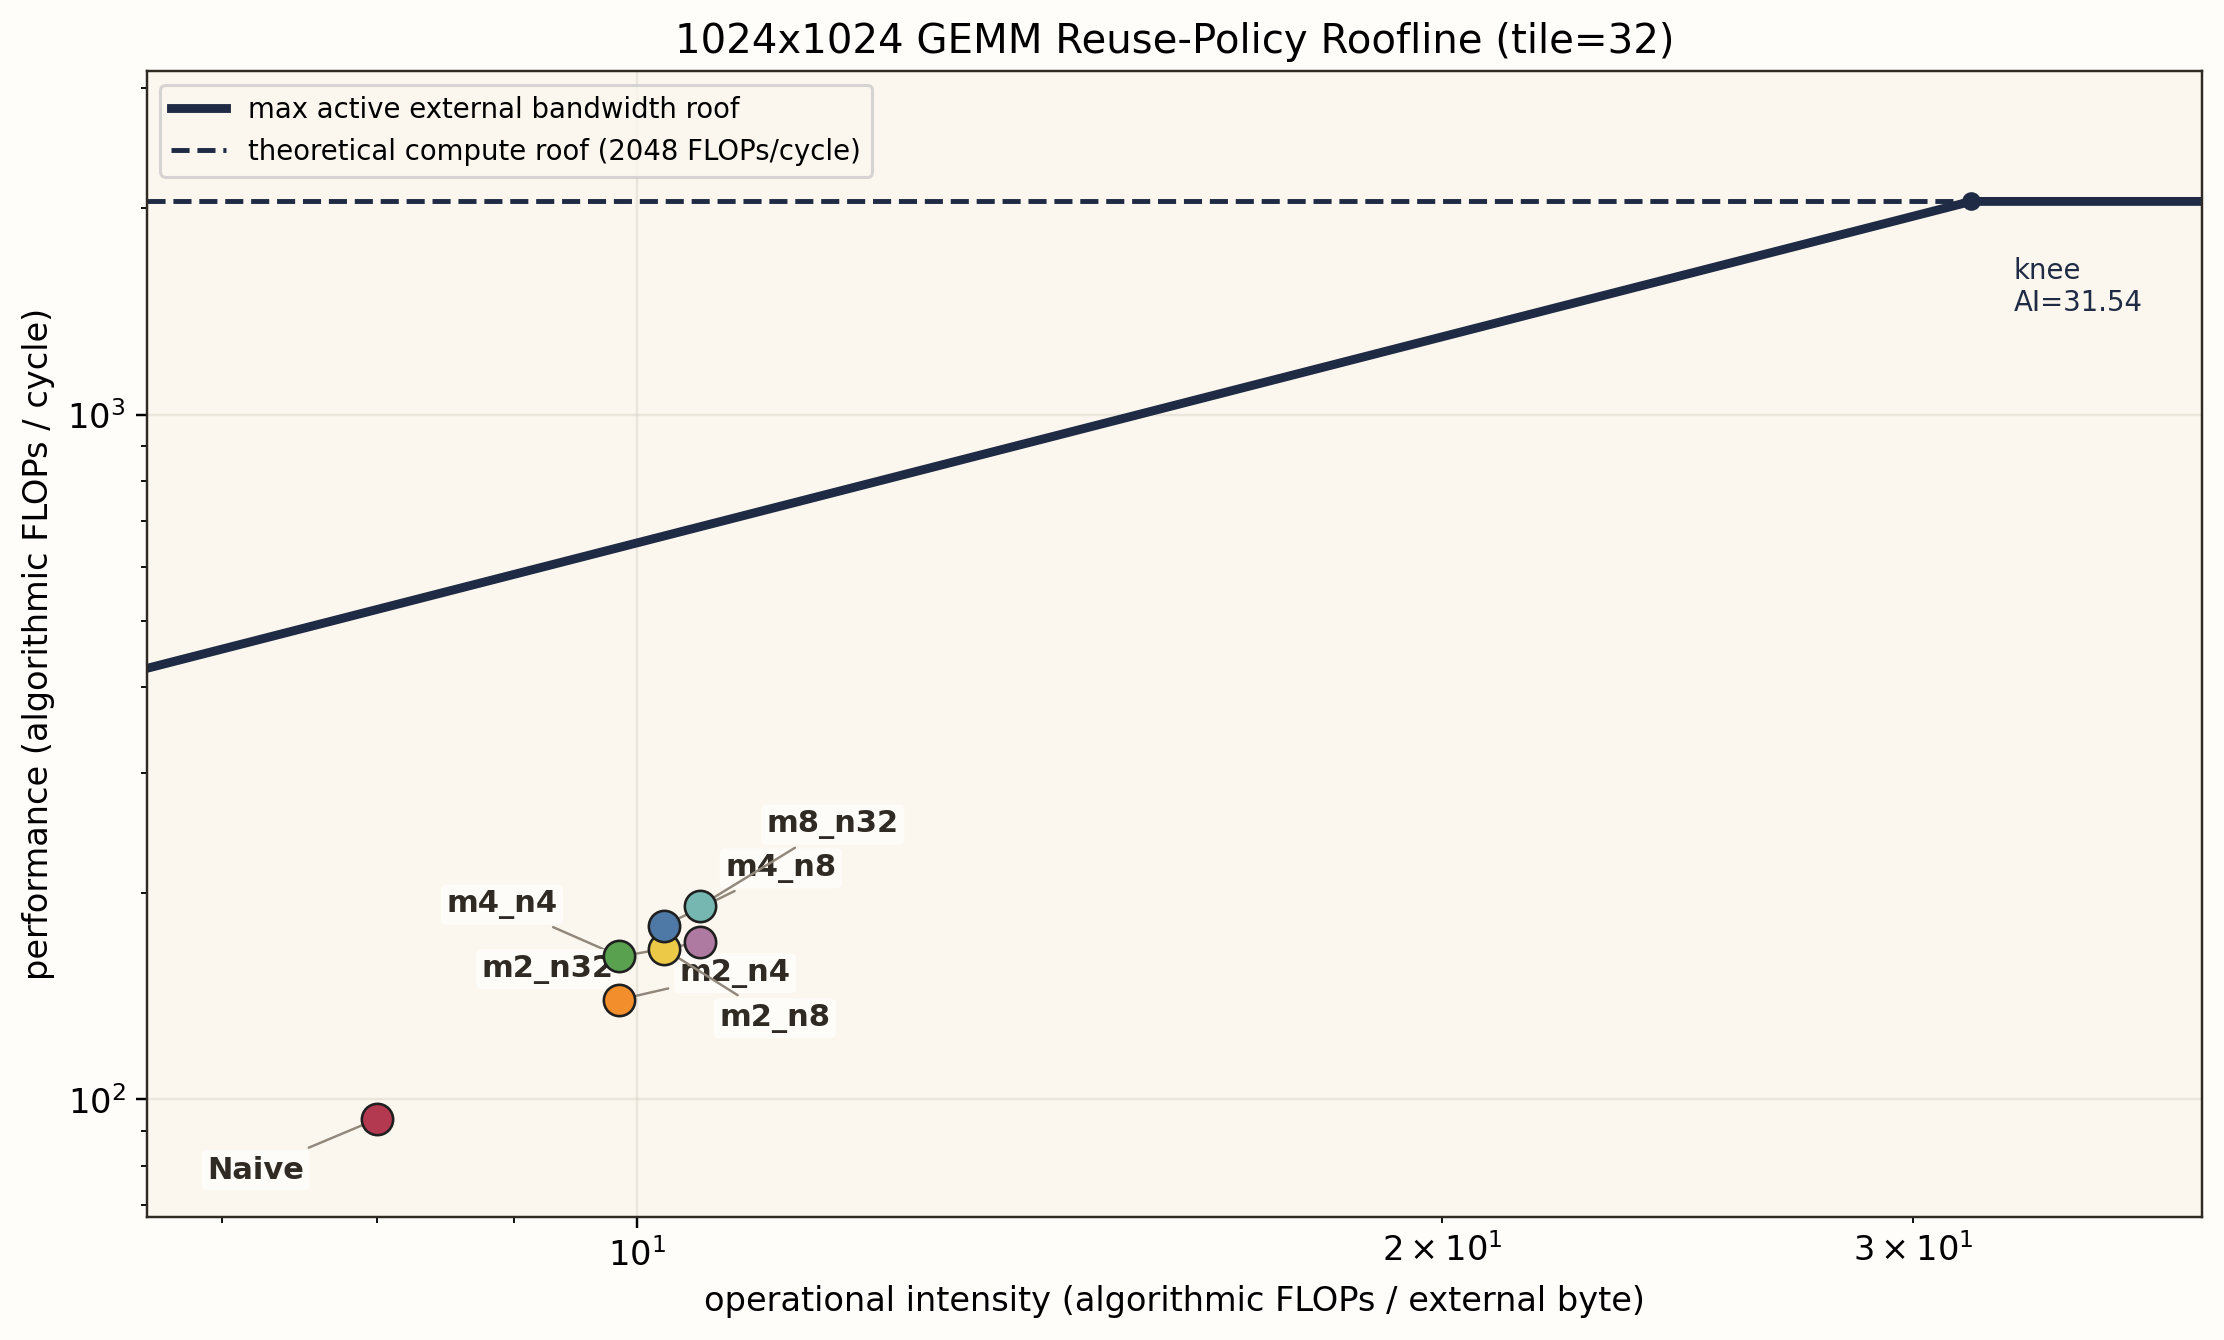
\includegraphics[width=\linewidth,height=.95\textheight,keepaspectratio]{figures/reuse_policy_roofline.png}
    \caption{Roofline plot for different tiling strategies, using $P(I)=\min(P_{\max}, B_{\max} I)$ with a systolic-array compute roof and an empirical active external-bandwidth roof.}
    \label{fig:roofline}
\end{figure}

\Cref{fig:roofline} is constructed from the standard roofline relation
$$
P(I) = \min(P_{\max}, B_{\max} I),
$$
where each plotted policy point uses the fixed algorithmic GEMM work for the numerator: $P = \frac{2N^3}{\text{cycles}}$ FLOP/cycle and $I = \frac{2N^3}{\texttt{bytes\_transmitted}}$ FLOP/B for the $1024\times1024$ GEMM. For this report, the compute roof is taken from the systolic array alone,
$$
P_{\max} = 2 \cdot \texttt{tile\_size}^2 = 2 \cdot 32^2 = 2048\ \text{FLOP/cycle},
$$
because a fully occupied $32\times32$ MAC array performs one multiply-accumulate per PE per cycle and each MAC counts as two floating-point operations. The bandwidth roof uses the maximum measured active external bandwidth across the compared runs, $B_{\max}=64.94$ B/cycle. This yields a roofline knee at about $\frac{2048}{64.94} \approx 31.5$ FLOP/B. If the model were extended to overlap vector-lane accumulation with systolic-array matmul and count that overlapped work in the same performance metric, then $P_{\max}$ would need to be redefined accordingly; the current roof uses only the matmul engine peak.

Under that construction, the naive baseline sits at roughly $(8.00\ \text{FLOP/B}, 93.66\ \text{FLOP/cycle})$. Moving to $m2\_n4$ and $m2\_n8$ shifts the operating point to the right as external bytes fall from 268M to 218M and then 210M, and upward as throughput rises to 139.78 and 165.86 FLOP/cycle. The $m4$ points show the complementary effect of weight residency: $m4\_n4$ and $m4\_n8$ have the same arithmetic intensities as the corresponding $m2$ points, but higher throughput, indicating that once bytes moved are fixed, additional resident weights improve how efficiently that traffic is converted into sustained compute.

The larger $n=32$ points continue this trend, reaching about 10.56 FLOP/B and 169.51 FLOP/cycle for $m2\_n32$ and 191.44 FLOP/cycle for $m8\_n32$. Even so, all of these points remain far below the 2048 FLOP/cycle compute roof and well left of the roofline knee at about 31.5 FLOP/B. The blocked policies therefore move the system in the right direction, but they do not bring it close to the compute roof. The measured gains remain bandwidth-limited improvements driven by traffic reduction and better overlap, not by any approach to peak arithmetic throughput.

\subsection{Evaluation Summary}
% summarize the baseline bottleneck, the effect of blocked reuse, and the new post-reuse limiter
% keep this to 3--4 direct takeaways tied to the measured results
% close by stating what the best measured policy demonstrates and what still prevents peak-compute operation

1- The tiled naive solution works correctly, but it is heavily preload- and accumulation-limited. Only about 10\% of total cycles fall inside valid-MAC windows, and even those windows fill the array to just 45.07\%, which is why the end-to-end MAC utilization is only 4.57\%.

2- Blocked reuse significantly reduces traffic and makes the compute bursts much denser. Compared to the naive solution, which generates 268M bytes of VLS-visible traffic, blocked policies reduce traffic first to 218M, then to 210M, and finally to 203M bytes while increasing throughput from 93.66 to a maximum of 191.44 FLOP/cycle and active-window MAC utilization from 45.07\% to 96.60\%.

3- Activation-side reuse reduces traffic more effectively than additional weight-side residency, but the latter remains important for sustaining higher throughput. The best measured point is $m8\_n32$ with queue size 4, reaching 11.22M cycles and a 2.04$\times$ speedup versus the naive baseline, but its full-run MAC utilization is still only 9.35\% because preload, psum reload/store, and queue/service overhead still consume roughly 90\% of total cycles.